\chapter[Resposta de PTA]{Resposta tensorial dispersiva de PTA e validação das correlações}
\label{chap:resposta-pta}

O objetivo deste capítulo é construir a resposta observacional do setor
tensorial e verificar sua integração sobre um fundo isotrópico. A
curvatura local obtida anteriormente não constitui, sozinha, um resíduo
de temporização. É necessário acompanhar a trajetória do fóton,
comparar as frequências medidas nos extremos e conservar as fases
relativas. As referências de validação são Liang--Trodden, na revisão
arXiv v3, e Cordes e colaboradores, na revisão v2
\autocite{liang2021,cordes2025}. Os resultados numéricos apresentados
referem-se à implementação e às configurações efetivamente executadas;
não constituem ainda uma campanha de inferência.

\section{Geometria e convenções de Fourier}

Sejam \(\hat p_a\) a direção da Terra para o pulsar \(a\),
\(L_a\) sua distância e \(\hat\Omega\) a direção de propagação
da onda. A direção aparente de origem da onda é, portanto,
\(-\hat\Omega\). Para \(f>0\), definem-se
\begin{equation}
 \begin{aligned}
 \omega&=2\pi f,&
 \beta&=\frac{ck}{\omega}=\sqrt{1-(f_g/f)^2},\\
 y_a&=\frac{2\pi fL_a}{c},&
 D_a&=1+\beta\mu_a,
 \qquad\mu_a=\hat\Omega\cdot\hat p_a.
 \end{aligned}
 \label{eq:pta-geometria}
\end{equation}
A função de resposta será escrita com fase
\(e^{i\omega(t-\beta\hat\Omega\cdot\mathbf x/c)}\), complexa
conjugada da escolha do capítulo anterior. A descrição de um campo
real é equivalente, mas a conjugação deve acompanhar os espectros
cruzados complexos. A razão \(\beta\) representa a velocidade de
grupo em unidades de \(c\); a velocidade de fase é \(c/\beta\).
Aqui \(f_g=m_gc^2/h_{\mathrm P}\), e as componentes de direções
espaciais e seus produtos escalares utilizam a métrica euclidiana.

A onda viajante exige \(f\geq f_g\). O código rejeita frequências
inferiores, em vez de substituir a raiz por seu módulo. No limiar,
\(\beta=0\), as expressões serão avaliadas por limites regulares.
Essa rejeição é o domínio de uma função de resposta de ondas
viajantes. O simulador futuro deverá decidir, explicitamente, como
representar um setor ausente abaixo do limiar; rejeitar um argumento
da função não equivale a excluir automaticamente uma hipótese física
inteira.

O pulso recebido na Terra no instante \(t\) percorre, na aproximação
não perturbada,
\begin{equation}
 \mathbf x(s)=s\hat p_a,\qquad t(s)=t-s/c,
 \qquad 0\leq s\leq L_a.
 \label{eq:pta-trajetoria}
\end{equation}
Sua fase no pulsar difere da terrestre por
\begin{equation}
 H_{ij}^{P}(t)=H_{ij}^{E}(t)e^{-iy_aD_a}.
 \label{eq:pta-fase-pulsar}
\end{equation}
O sinal positivo em \(D_a\) decorre de o fóton viajar no sentido
\(-\hat p_a\). Empregar a direção da fonte no lugar da direção de
propagação sem modificar o denominador inverteria essa convenção.

\section{Desvio de frequência e resíduo de temporização}

No setor TT, \(H_{0\mu}=0\), e observadores espacialmente fixos
nessas coordenadas são geodésicos à ordem considerada. Com
\(\eta=(+---)\), a equação do momento covariante do fóton é
\begin{equation}
 \frac{dp_0}{d\lambda}
 =\frac12\partial_0 H_{ij}\,p^ip^j.
 \label{eq:pta-foton}
\end{equation}
Na trajetória de ordem zero, \(p^i=-p^0\hat p_a^i\). Além disso,
a derivada total da onda ao longo do fóton satisfaz
\(dH_{ij}/dt=D_a\partial_tH_{ij}\). Integrar
\eqref{eq:pta-foton} entre emissão e recepção produz
\begin{equation}
 \frac{\nu_E-\nu_P}{\nu_P}
 =\frac{\hat p_a^i\hat p_a^j}{2D_a}
              (H_{ij}^{E}-H_{ij}^{P}).
 \label{eq:pta-ganho-frequencia}
\end{equation}
Aqui \(H_{ij}\) é a perturbação \emph{covariante} espacial usada
no capítulo anterior, após a mudança da convenção de Fourier.

Para conservar o significado usual de atraso positivo no resíduo,
define-se \(z_a=(\nu_P-\nu_E)/\nu_P\) e
\(r_a(t)=\int^t z_a(t')\,dt'\). O código armazena o núcleo
geométrico positivo
\begin{equation}
 R_a^A=
 \frac{\hat p_a^i\hat p_a^je_{ij}^A}{2D_a}
             (1-e^{-iy_aD_a}),
 \qquad A\in\{+,\times\},
 \label{eq:pta-nucleo}
\end{equation}
com \(e_{ij}^Ae_{ij}^B=2\delta_{AB}\). A resposta do redshift
definido acima é \(-R_a^A\). Esse sinal global desaparece de
produtos \(R_aR_b^*\), mas deve ser mantido ao produzir séries
temporais. Para \(f\ne0\),
\begin{equation}
 \widetilde r_a(f)=\frac{\widetilde z_a(f)}{i2\pi f}.
 \label{eq:pta-residuo}
\end{equation}
A constante de integração e a projeção do modelo de temporização
serão tratadas na modelagem dos dados, não como parte da ORF.

Os termos 1 e exponencial de \eqref{eq:pta-nucleo} correspondem,
respectivamente, à Terra e ao pulsar. Sua combinação deve ser avaliada
antes de uma divisão numericamente delicada. Introduzindo
\begin{equation}
 g(y,D)=\frac{1-e^{-iyD}}{D}
       =iy\,e^{-iyD/2}\operatorname{sinc}(yD/2),
 \label{eq:pta-transferencia}
\end{equation}
com \(\operatorname{sinc}u=\sin u/u\), obtém-se
\(g(y,0)=iy\). Assim, o ponto \(D=0\), possível em
\(\beta=1\), \(\mu=-1\), é removível na resposta completa.
Não é necessário recortar uma região angular ao redor desse ponto.
A implementação considera que a função \texttt{numpy.sinc} utiliza
\(\sin(\pi u)/(\pi u)\), ajustando seu argumento.

\subsection{Componentes temporais e observadores livres}

O tratamento TT não autoriza manter os observadores espacialmente
fixos quando \(H_{0\mu}\ne0\). Na nossa assinatura, em \(c=1\)
e com constantes homogêneas de movimento escolhidas nulas, a
normalização e a equação geodésica dão
\begin{equation}
 \delta u^0=-\frac{H_{00}}2,\qquad
 \delta u^i=H_{0i}+\frac{\beta\Omega_i}{2}H_{00}.
 \label{eq:pta-observadores}
\end{equation}
A frequência local é a contração do momento com a quatro-velocidade.
Somar sua correção nos extremos à variação do momento do fóton
organiza o numerador em
\begin{equation}
 Q_{ij}=H_{ij}+\beta\Omega_iH_{0j}
              +\beta\Omega_jH_{0i}
              +\beta^2\Omega_i\Omega_jH_{00}.
 \label{eq:pta-q-geral}
\end{equation}
O ganho fracionário contém
\(\hat p^i\hat p^j(Q_{ij}^{E}-Q_{ij}^{P})/(2D)\).
Para uma onda plana na convenção de curvatura anterior,
\(Q_{ij}=2R_{0i0j}/\omega^2\), em unidades \(c=1\).
O cancelamento decorre da trajetória e das frequências locais, não de
uma substituição arbitrária de amplitudes de maré por amplitudes de
resposta.

A seção III da revisão v3 de Liang--Trodden inclui precisamente a
necessidade de corrigir o movimento dos observadores; seu termo
proporcional a \(\epsilon_{00}\) na equação (22) desaparece em TT
\autocite{liang2021}. As equações
\eqref{eq:pta-observadores}--\eqref{eq:pta-q-geral} explicitam a
tradução preparatória de convenções. Os benchmarks deste capítulo
avaliam o setor tensorial; não validam uma população escalar ou
vetorial, que exigirá implementação própria.

\section{ORF e normalização espectral}

Define-se, para a população tensorial isotrópica e não polarizada,
\begin{equation}
 \Gamma_{ab}(f)=\frac{3}{8\pi}\int d^2\hat\Omega
             \sum_A R_a^A R_b^{A*}.
 \label{eq:pta-orf-definicao}
\end{equation}
A normalização é fixa: no limite GR de grandes distâncias, a
autocorrelação tende a um. Para pulsares distintos cujos termos
individuais sejam incoerentes, o limite de separação angular nula da
contribuição terrestre é \(1/2\). Não se impõe diagonal unitária
para toda massa e distância; fazê-lo pode absorver dependência física
em uma redefinição do espectro e da priori de amplitude.

Uma convenção consistente para os coeficientes do campo é
\begin{equation}
 \begin{aligned}
 \langle\widetilde h_A(f,\Omega)
        \widetilde h_{A'}^*(f',\Omega')\rangle
 ={}&\frac{S_h(|f|)}{8\pi}\delta_{AA'}\delta(f-f')\\
   &\times\delta^2(\Omega,\Omega').
 \end{aligned}
 \label{eq:pta-espectro-campo}
\end{equation}
A convenção de \(S_h\), correspondente à equação (3) de
Cordes \autocite{cordes2025}, somada ao fator dois que
converte a correlação bilateral em espectro unilateral, fornece
\begin{equation}
 S_{ab}^{r}(f)
 =\frac{\Gamma_{ab}(f)S_h(f)}{6\pi^2f^2}
 =\frac{\Gamma_{ab}(f)h_c^2(f)}{12\pi^2f^3},
 \qquad h_c^2(f)=2fS_h(f).
 \label{eq:pta-espectro-residuos}
\end{equation}
As dimensões são \([S_h]=\mathrm{s}\) e
\([S^r]=\mathrm{s}^3\). Não foi assumida uma relação com densidade
de energia gravitacional de uma teoria completa. Para confrontar
Liang--Trodden, cujas polarizações circulares têm norma unitária, seu
coeficiente de normalização \(\beta_T\) deve ser
\(3/(4\pi)\). Esse símbolo não é a velocidade \(\beta\) do
presente projeto. A mudança de base e norma explica o fator dois.
A comparação utiliza a equação (35) e a definição algébrica de
normalização no texto de Liang--Trodden \autocite{liang2021}.

Em geral, \(\Gamma_{ba}=\Gamma_{ab}^*\). Sua matriz é positiva
semidefinida, pois, para qualquer vetor complexo \(v\),
\begin{equation}
 v^\dagger\Gamma v
 =\frac{3}{8\pi}\int d^2\hat\Omega\sum_A
          \left|\sum_a v_a^*R_a^A\right|^2\geq0.
 \label{eq:pta-positividade}
\end{equation}
Distâncias diferentes podem produzir partes imaginárias não nulas.
Descartá-las exige uma média ou aproximação declarada. Autovalores
negativos relevantes em uma aproximação numérica devem motivar
investigação de convergência e normalização, não uma correção
automática que esconda o problema.

\section{Duas rotas de integração angular}

\subsection{Projetor TT e quadratura direta}

Se \(P_{ij}=\delta_{ij}-\Omega_i\Omega_j\), a soma de
polarizações reais TT satisfaz
\begin{equation}
 \sum_A e_{ij}^Ae_{kl}^A
       =P_{ik}P_{jl}+P_{il}P_{jk}-P_{ij}P_{kl}.
 \label{eq:pta-projetor-tt}
\end{equation}
Sua contração com as direções dos pulsares produz
\begin{equation}
 \mathcal T_{ab}
 =2(\delta-\mu_a\mu_b)^2
       -(1-\mu_a^2)(1-\mu_b^2),
 \qquad\delta=\hat p_a\cdot\hat p_b.
 \label{eq:pta-soma-tensorial}
\end{equation}
Esse procedimento evita introduzir um referencial transversal
singular em algum ponto do céu. Escolhendo
\(\hat p_a=(0,0,1)\), \(\hat p_b=(\sin\zeta,0,\cos\zeta)\)
e \(x=\cos\theta\), tem-se
\begin{equation}
 \mu_a=x,\qquad
 \mu_b=\delta x+\sqrt{1-\delta^2}\sqrt{1-x^2}\cos\varphi.
 \label{eq:pta-mu-b}
\end{equation}
Portanto,
\begin{equation}
 \Gamma_{ab}=\frac{3}{32\pi}
 \int_{-1}^{1}dx\int_0^{2\pi}d\varphi\,
 \mathcal T_{ab}\,g(y_a,D_a)g^*(y_b,D_b).
 \label{eq:pta-integral-direta}
\end{equation}
A implementação combina Gauss--Legendre em \(x\) com trapézios
periódicos em \(\varphi\). O azimute é processado em blocos para
controlar a memória, preservando os mesmos nós e pesos. No modelo
apenas Terra, cada \(g\) é substituído por \(1/D\).

\subsection{Expansão harmônica e truncamento}

Uma segunda rota expande a resposta individual em funções associadas
de Legendre. Para \(\ell\geq2\),
\begin{equation}
 c_\ell(\beta,y)=\int_{-1}^{1}dx\,
     (1-x^2)^2P_\ell''(x)g(y,1+\beta x).
 \label{eq:pta-coeficientes}
\end{equation}
A identidade \(P_\ell^2=(1-x^2)P_\ell''\) e a ortogonalidade
\begin{equation}
 \int_{-1}^{1}P_\ell^2(x)P_j^2(x)\,dx
 =\frac{2(\ell+2)!}{(2\ell+1)(\ell-2)!}\delta_{\ell j}
 \label{eq:pta-ortogonalidade}
\end{equation}
fixam a normalização dos coeficientes. O teorema de adição aplicado à
rotação entre direções fornece
\begin{equation}
 \Gamma_{ab}=\frac3{32}\sum_{\ell=2}^{\infty}
 \frac{(2\ell+1)c_\ell(\beta,y_a)c_\ell^*(\beta,y_b)}
 { (\ell-1)\ell(\ell+1)(\ell+2)}P_\ell(\delta).
 \label{eq:pta-serie-harmonica}
\end{equation}
Para distâncias iguais, recuperam-se as equações (15)--(16) de
Cordes \autocite{cordes2025}; para
distâncias diferentes, o produto cruzado conserva a fase. Essa forma
foi confrontada com \eqref{eq:pta-integral-direta}, sem substituir
indevidamente o produto por um módulo ao quadrado.

A recorrência de \(P_\ell^2\) permite reutilizar termos adjacentes.
Dois controles permanecem distintos: o número de nós que calcula
\(c_\ell\) e o corte \(\ell_{\max}\) da soma. Refinar apenas
um pode deixar o outro como fonte dominante de erro. Em uma rede,
os coeficientes de cada pulsar podem ser calculados uma vez por
frequência e reutilizados nos pares, desde que as configurações de
quadratura satisfaçam a precisão exigida.
Um corte harmônico comum preserva a positividade da matriz: pelo
teorema de adição, cada multipolo é uma soma de produtos de
amplitudes complexas e seus conjugados. Escolher cortes diferentes
independentemente para cada par não assegura essa propriedade.
Além disso, positividade semidefinida não implica invertibilidade;
direções coincidentes e o limiar podem produzir autovalores nulos
físicos. A montagem da covariância exigirá examinar também seu
condicionamento.

\section{Limites analíticos e ordem das aproximações}

\subsection{Hellings--Downs e autocorrelação}

No caso GR apenas Terra, integrar por partes
\eqref{eq:pta-coeficientes} fornece
\(c_\ell=4(-1)^\ell\). Os termos interiores restantes contêm
polinômios de grau inferior a dois, ortogonais a \(P_\ell\) para
\(\ell\geq2\). Sua soma recupera
\begin{equation}
 \Gamma_{\mathrm{HD}}(\zeta)
 =\frac12-\frac{u}{4}+\frac32u\ln u,
 \qquad u=\frac{1-\cos\zeta}{2},
 \label{eq:pta-hd}
\end{equation}
com \(u\ln u=0\) em \(u=0\). A autocorrelação completa não é
obtida impondo essa curva na diagonal. Com \(y=2\pi fL/c\),
\begin{equation}
 \Gamma_{aa}^{\mathrm{GR}}(y)
 =1-\frac{3}{2y^2}\left[1-\frac{\sin(2y)}{2y}\right].
 \label{eq:pta-auto-gr}
\end{equation}
Essa expressão, equivalente à equação (25) de Cordes, tende a um
para grandes \(y\). Para \(y\to0\), sua forma estável é
\(y^2/5-2y^4/105+y^6/945+O(y^8)\).

Para massa não nula e distância finita, uma verificação independente
é a integral unidimensional
\begin{equation}
 \Gamma_{aa}(\beta,y)
 =\frac3{16}\int_{-1}^{1}(1-x^2)^2
                  |g(y,1+\beta x)|^2\,dx.
 \label{eq:pta-auto-integral}
\end{equation}
O algoritmo separa as partes constante e oscilatória e usa
quadratura adaptativa com pesos seno e cosseno em fases grandes.
Em fases pequenas, integra a forma estável diretamente. Para
\(y\to\infty\), a \(0<\beta<1\) fixo, resulta
\begin{equation}
 \Gamma_{aa}^{\mathrm{assint}}=
 \frac{6\beta-4\beta^3+
  3(\beta^2-1)\ln[(1+\beta)/(1-\beta)]}{2\beta^5}.
 \label{eq:pta-auto-assintotica}
\end{equation}
Esse resultado de Cordes tende a \(2/5\) quando
\(\beta\to0\), mas essa ordem de limites não é uniforme.

\subsection{Limiar, coerência e separação pequena}

Em \(\beta=0\), a transferência deixa de depender da direção.
Somente o quadrupolo contribui, com \(c_2^{EE}=16/5\), e
\begin{equation}
 \begin{aligned}
 \Gamma_{ab}^{EE}&=\frac15P_2(\cos\zeta),\\
 \Gamma_{ab}&=(1-e^{-iy_a})(1-e^{iy_b})
                         \frac15P_2(\cos\zeta),\\
 \Gamma_{aa}&=\frac45\sin^2(y_a/2).
 \end{aligned}
 \label{eq:pta-limiar}
\end{equation}
A última linha oscila quando \(y\) cresce e não possui limite
pontual constante. Assim, \(fL/c\gg1\), isoladamente, não garante
incoerência perto do limiar. A escala angular da fase individual é
\(\beta y\), enquanto a fase pulsar--pulsar envolve o vetor
\begin{equation}
 \mathbf b_{ab}=\beta(y_a\hat p_a-y_b\hat p_b).
 \label{eq:pta-coerencia-par}
\end{equation}
Se seu módulo é pequeno, a média angular pode preservar a correlação
entre os termos dos pulsares. A ORF finita é contínua quando suas
posições tendem uma à outra. O salto aproximado entre \(1/2\) e
1 no limite HD representa a hipótese de incoerência e a ordem dos
limites, não uma descontinuidade da resposta finita.

Incertezas de distância, largura dos canais e médias de fase podem
suprimir essa coerência. Tais médias precisam ser realizadas no
modelo observacional. Os exemplos a distâncias e frequências fixas
não demonstram que correções grandes sobrevivam em toda PTA real.
Para a resposta apenas Terra, uma expansão regular adicional é
\begin{equation}
 \Gamma^{EE}(\beta,\delta)
 =\frac{P_2(\delta)}5+
   \frac{\beta^2}{35}[2P_2(\delta)+P_3(\delta)]+O(\beta^4).
 \label{eq:pta-expansao-limiar}
\end{equation}
O código utiliza essa série para \(\beta<10^{-4}\), evitando
cancelamento na fórmula fechada. Para os demais valores interiores,
a expressão analítica apenas Terra é avaliada com 90 dígitos
decimais; os casos \(\beta=0,1\) e \(\delta=1\) recebem
limites próprios. Essa estabilidade algébrica não substitui o
controle das integrais oscilatórias da resposta completa.

\section{Benchmarks executados e orçamento de erro}

A implementação integrada foi executada com NumPy 2.4.3 e SciPy 1.17.1.
Seus 23 testes incluem oito verificações de domínio, transferência,
limites, integrações e normalização; quatro testes físicos independentes;
e onze controles de entradas, orçamento e convergência da interface. Uma campanha de 20 configurações selecionadas, com
\(\zeta=\pi/8\), comparou a integral direta à série refinada.
Os valores de \(fL/c\) foram \(0{,}125\), \(1{,}125\),
\(10{,}125\), \(100{,}125\) e \(1000{,}125\), com
\(\beta=0\), \(0{,}01\), \(0{,}9\) e 1; no último grupo,
o caso exatamente nulo foi substituído por \(\beta=10^{-5}\).
A maior diferença absoluta entre métodos foi
\(2{,}94\times10^{-13}\). Esses pontos não certificam um domínio
contínuo com a mesma tolerância.

Uma auditoria acrescentou quatro testes físicos independentes. Foi
construído um céu comum para seis pulsares, com polarizações TT
explícitas, direções gerais e um par quase coincidente. Nas fases
entre 19 e 90 utilizadas nesses testes, a diferença máxima para a
matriz harmônica foi \(4{,}43\times10^{-14}\), e a variação
sob uma rotação global foi \(4{,}85\times10^{-14}\). O menor
autovalor, aproximadamente \(-2{,}28\times10^{-15}\), foi
compatível com arredondamento. Também foram verificadas a
continuidade na coincidência e a extensão
\(\Gamma(-f)=\Gamma(f)^*\), necessária para construir uma
covariância real no tempo. Esses controles testam geometria e
convenções por uma construção distinta; suas resoluções moderadas
não certificam as fases maiores da campanha principal.

A tabela apresenta valores arredondados, para distâncias iguais.
Nesses casos, a parte imaginária é compatível com zero. A diferença
entre resposta completa e apenas Terra é uma diferença de modelos,
não uma estimativa de erro numérico.

\begin{center}
\begingroup\small\singlespacing
\setlength{\tabcolsep}{5pt}
\begin{tabular}{@{}rrccc@{}}
\toprule
\(\beta\) & \(fL/c\) & \(\Gamma\) completa &
\(\Gamma^{EE}\) & \(\Gamma_{aa}\) completa\\
\midrule
0 & \(100{,}125\) & \(0{,}091421\) & \(0{,}156066\) & \(0{,}117157\)\\
\(0{,}01\) & \(100{,}125\) & \(0{,}163339\) & \(0{,}156072\) & \(0{,}408063\)\\
\(0{,}9\) & \(100{,}125\) & \(0{,}248374\) & \(0{,}247005\) & \(0{,}682204\)\\
1 & \(100{,}125\) & \(0{,}304472\) & \(0{,}303880\) & \(0{,}999996\)\\
\(10^{-5}\) & \(1000{,}125\) & \(0{,}091462\) & \(0{,}156066\) & \(0{,}117237\)\\
\(0{,}01\) & \(1000{,}125\) & \(0{,}149081\) & \(0{,}156072\) & \(0{,}400018\)\\
\(0{,}9\) & \(1000{,}125\) & \(0{,}247161\) & \(0{,}247005\) & \(0{,}682204\)\\
1 & \(1000{,}125\) & \(0{,}304026\) & \(0{,}303880\) & \(1{,}000000\)\\
\bottomrule
\end{tabular}
\endgroup
\end{center}

Uma segunda campanha contém 16 casos próximos da coincidência,
com \(\beta=0{,}9\) ou 1, separações
\(0,10^{-5},10^{-3},10^{-2}\) radianos e distâncias iguais ou
diferentes. Sua maior diferença absoluta entre métodos foi
\(5{,}25\times10^{-12}\). Para ilustrar a fase preservada, em
\(\beta=1\), separação zero,
\(fL_a/c=1000{,}125\) e
\(fL_b/c=1000{,}125+1/(2\pi)\), obteve-se
\begin{equation}
 \Gamma_{ab}\simeq0{,}90901343+0{,}21894496\,i.
 \label{eq:pta-exemplo-complexo}
\end{equation}
Os pulsares ocupam a mesma direção, mas não a mesma posição; esse
caso não é uma autocorrelação. Conjugar a convenção de Fourier troca
o sinal da parte imaginária, como exige a consistência das convenções.

Nas duas raízes de Hellings--Downs, próximas de
\(49{,}3173^\circ\) e \(121{,}7889^\circ\), os erros absolutos
da integral terrestre foram \(1{,}84\times10^{-7}\) e
\(1{,}66\times10^{-7}\). Ambos estão abaixo da tolerância
absoluta inicial de \(10^{-5}\). Erro relativo não é uma medida
adequada exatamente em uma raiz. Fora delas, a tolerância relativa
inicial do plano é \(10^{-3}\), a ser propagada posteriormente
para o orçamento de erro da inferência.

\subsection{Resolução necessária e limites da validação}

Os resultados precisos acima utilizaram resoluções específicas e
refinamento. Resoluções insuficientes podem retornar números plausíveis. Por exemplo,
na autocorrelação GR
com \(fL/c=1000{,}125\), os valores aproximados
\(0{,}50035\) para uma série truncada em \(\ell_{\max}=200\)
e \(0{,}92907\) para quadratura direta \(200\times400\).
O valor analítico é \(0{,}999999962\). A discrepância representa
sub-resolução, não uma falha do limite físico.

A escolha inicial dos benchmarks escalou como
\(\ell_{\max}\approx\beta\max(y_a,y_b)+90\) e refinou
também os nós da integração. Essa regra é empírica; o resultado deve
ser aceito somente após conferir estabilidade ao aumentar
quadratura e truncamento separadamente. Para
\(\beta=1\), \(fL/c=1000{,}125\), a campanha principal utilizou
\(\ell_{\max}=6373\), 12757 nós para os coeficientes e uma
quadratura direta de \(7660\times6011\) pontos. As resoluções
refinadas e suas diferenças constam dos JSONs de benchmark.

Nessa máquina, uma avaliação harmônica desse caso custou cerca de
2,34 segundos, e a direta, 1,67 segundo. Esses tempos dependem de
hardware, cache e configuração; não são uma promessa de custo para
qualquer rede. O crescimento relevante acompanha \(\beta fL/c\)
e a resolução das correlações entre posições próximas. A campanha
não certifica distâncias arbitrariamente grandes, todas as geometrias
ou a estabilidade de cada configuração sob qualquer priori.

\subsection{Contrato de aceitação da implementação}

A interface \texttt{pta.checked\_orf} exige resoluções grossa e fina,
um orçamento de trabalho e memória e tolerâncias absoluta e relativa.
Compara separadamente o refinamento dos nós harmônicos, o aumento de
\(\ell_{\max}\), o refinamento da quadratura direta e o acordo entre
métodos. Para apenas Terra, utiliza a referência analítica. Todos os
critérios devem satisfazer
\begin{equation}
 \epsilon_j\leq\epsilon_{\mathrm{abs}}
                   +\epsilon_{\mathrm{rel}}\lvert\Gamma_{ab}\rvert.
 \label{eq:pta-aceitacao}
\end{equation}
A ausência de convergência gera uma falha com diagnóstico. Não há
crescimento automático das resoluções: uma nova tentativa exige um novo
orçamento explícito. As estimativas de trabalho e memória são recursos
aproximados de planejamento, não limites rigorosos de tempo ou memória
residente. O acordo por refinamento também é um critério empírico,
não uma prova de erro absoluto para todo o domínio contínuo.

As entradas rejeitam valores não finitos, produtos escalares fora de
\([-1,1]\), fases negativas e uma única fase ausente. As ordens de
quadratura são inteiros positivos. O envelope de fase aceito é
\(0\leq y\leq2\pi\,1000{,}125+1\), cobrindo as duas campanhas;
as ordens têm teto de 20000. Pontos dentro desse envelope continuam
sujeitos às verificações de convergência. As funções numéricas de baixo
nível têm o prefixo \texttt{raw\_}, exigem resolução e não conferem
aceitação por si mesmas. O teste da auto GR sub-resolvida é recusado
pela interface, apesar de seu resultado bruto ser finito.

A campanha de aceitação integrada acrescentou refinamento separado em
58 casos: os 20 pares principais, 16 casos de coerência, 20 autos e dois
zeros de Hellings--Downs. Todos passaram. Os máximos absolutos entre os
controles foram, respectivamente,
\(1{,}38\times10^{-12}\), \(5{,}36\times10^{-12}\),
\(3{,}81\times10^{-12}\) e \(1{,}63\times10^{-6}\).
O confronto das autos com a referência unidimensional teve diferença
máxima de \(7{,}05\times10^{-13}\). A configuração exige também
cada erro absoluto abaixo de \(10^{-5}\) e, fora da vizinhança de
zero \(\lvert\Gamma\rvert\leq10^{-5}\), relativo abaixo de
\(10^{-3}\); esses critérios são mais estritos que a soma em
\eqref{eq:pta-aceitacao}.

Nos zeros HD, o erro direto não decresceu monotonicamente: no primeiro,
a malha fina produziu aproximadamente \(-1{,}44\times10^{-6}\),
enquanto a grossa produziu \(1{,}84\times10^{-7}\). Ambas passaram
pela tolerância absoluta, assim como sua diferença. Não se pressupõe
monotonicidade nem se seleciona apenas a malha com resultado mais
próximo de zero. A execução completa levou 64,82 segundos nesta máquina,
com cache de nós compartilhado; os hashes de fontes e configuração
permaneceram inalterados. O registro de 58 casos é separado das campanhas
iniciais e pode ser reconstituído pelo script do repositório.

\begin{figure}[htbp]
 \centering
 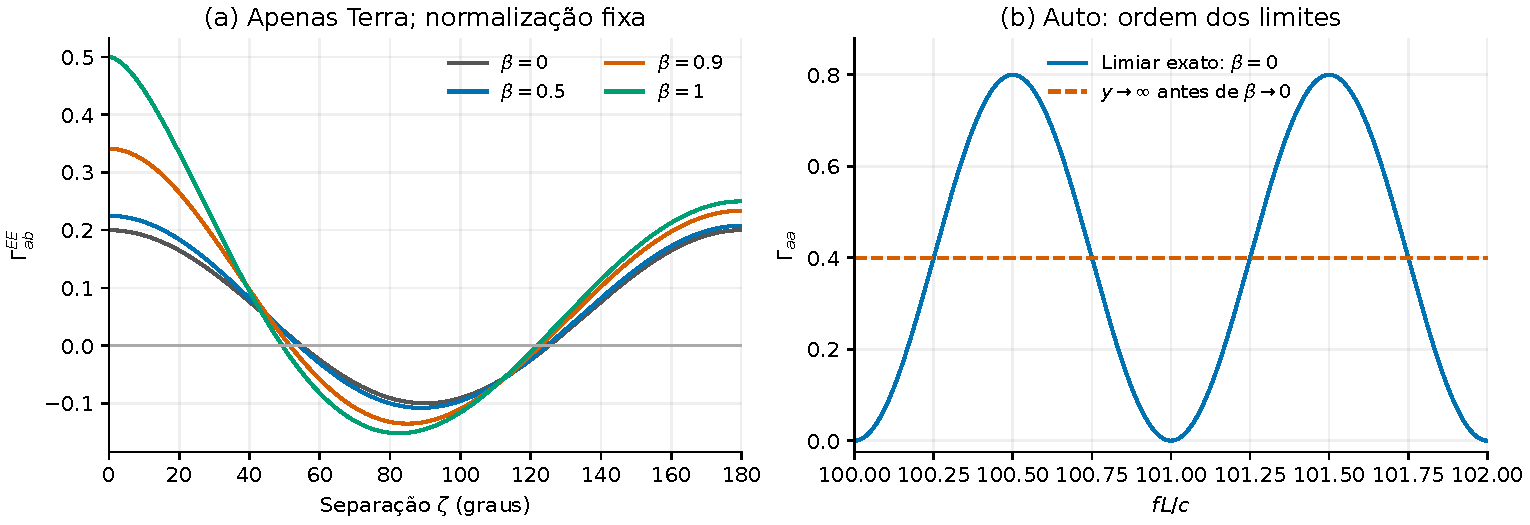
\includegraphics[width=\textwidth]{../figures/C05/orf_limites.pdf}
 \caption{Limites analíticos da resposta tensorial. À esquerda, a
 contribuição apenas Terra varia com \(\beta\) sob uma normalização
 fixa; \(\beta=1\) recupera Hellings--Downs. À direita, a auto no
 limiar exato conserva oscilações mesmo em \(fL/c\) grande. A linha
 tracejada representa a ordem inversa dos limites. As curvas são
 calculadas das expressões deste capítulo, sem médias em distância ou
 frequência e sem uma interpretação como dados observados.}
 \label{fig:pta-limites}
\end{figure}
A Figura~\ref{fig:pta-limites} distingue a mudança do modelo da
incerteza numérica. Seu código de geração e o arquivo vetorial integram
o release; a precisão dos benchmarks é examinada nos registros de
validação separados.

\section{Passagem para o simulador e alcance científico}

Os resultados estabelecem uma implementação tensorial com
normalização rastreável, dois métodos de integração e limites
analíticos compatíveis. Os módulos integrados de C05 validam o domínio
das entradas e exigem resoluções explícitas; a interface de aceitação
retorna também o relatório de refinamento. Uma
função que retorna um número finito não oferece, por esse fato,
garantia de convergência. Tampouco a concordância de duas integrações
da resposta completa valida automaticamente sua substituição pela
contribuição terrestre e uma diagonal assintótica.

O simulador de C06 deverá utilizar os mesmos espectros, fases e
convenções de covariância. Se incorporar médias em distância ou
frequência, elas deverão atuar no modelo e na estatística de maneira
compatível. A positividade de \eqref{eq:pta-positividade} será um
controle de construção da covariância, e a parte imaginária deverá
ser conservada quando pertinente. A eventual aproximação por termos
incoerentes precisa ser validada nas escalas
\(\beta y\) e \(\lvert\mathbf b_{ab}\rvert\) utilizadas.

Não foram inferidas massas, medidas coberturas ou detectadas
polarizações adicionais nesta etapa. O campo gaussiano, isotrópico e
TT é uma hipótese de população; a geração astrofísica e a relação
entre potência tensorial e setores adicionais permanecem separadas.
As campanhas posteriores deverão quantificar se erros residuais de
ORF e as aproximações de coerência são pequenos diante da
sensibilidade estatística. Esse teste liga a validação numérica à
pergunta de pesquisa, sem confundir precisão de uma integral com
validade de uma inferência.
